\chapter{Data Collection and Results}
\label{sec:results}


With a theoretical proof of the core of our algorithm complete, we can
move on to an analysis of its real-world implementability and
performance. We can first look at whether the tools we use to simulate
time synchronization in the real world continue to conform to the
invariant set out in our proof. We also can look at the performance of
our freezing algorithm and analyze how big of a freeze window is
necessary in a real world setting.

\section{Collection of NTP Performance in a Real-World Setting}

There are two primary characteristics of our algorithm that need
testing: the existence of the freeze period overlaps described in our
solution, and the worst and average case duration of these freeze
periods. As described above, we used simulations to observe the
existence of the overlap. In order to accurately simulate the
characteristics of a real Ceph cluster, we need to model the actual
behavior of a given Ceph cluster.

To do so, we used the Network Time Protocol daemon, ntpd, which is an
operating system program that maintains the system time in
synchronization with the Network Time Protocol (NTP) servers. This
allowed us to log data and statistics about the clock and network
communications. In particular, the data that interests us for
simulation is the clock jitter and network latency.

The clock jitter is the estimated random error on a given computer's
clock drift from the NTP server, and is typically measured in Parts
Per Million (PPM). For example, a PPM of 10 for clock jitter would
mean for every million clock ticks of the NTP server, the local
computer could be off by 10 ticks. The network latency is a measure of
the round trip time of the message passed between the local computer
to the NTP server and back. This is typically on the order of
milliseconds. <TODO citation> <development>

The Ceph test cluster includes three types of computers named Mira,
Plana, and Burnupi. Miras and Planas use Intel-based chips, while
Burnupi uses AMD chips.

The histogram on figure~\ref{fig:latency-hist} shows the collected
values on network latency. Note that there are three peaks that can be
seen, and this is reflective of the three different types of
computers. Among all three types of computers, network latency in the
test cluster appear to generally be around single digit milliseconds.

\begin{figure}[h]
  \centering
  \caption{Histogram of network latency across 235 nodes in a Ceph test cluster.} 
  %% TODO add stats when more accurate graphs 
  %% are generated (hopefully without 3 peaks)
  \label{fig:latency-hist}
  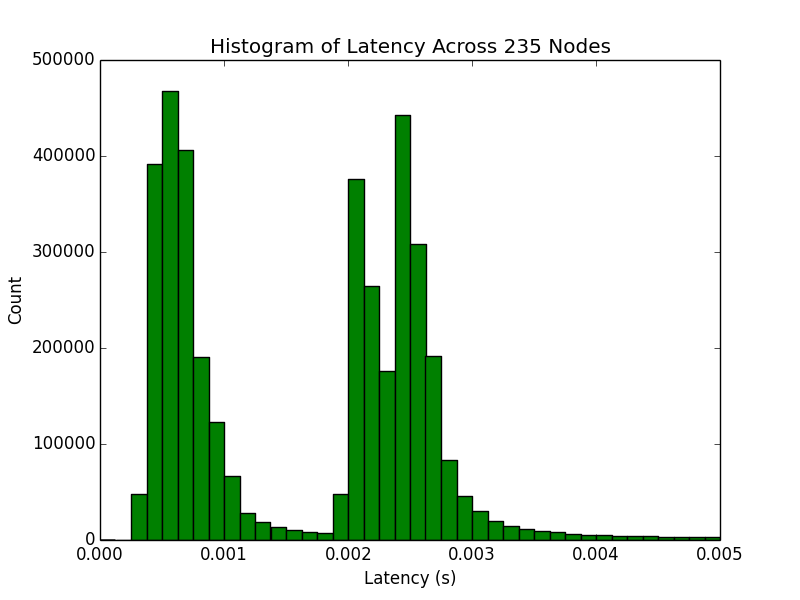
\includegraphics[width=0.8\textwidth]{latency-hist.png}
\end{figure}


We observed the behavior of clock jitter on the same Ceph test
cluster, as shown in Figure A, B, and C for the different types of
computers. Despite the different offsets, these can be seen to have a
generally normal distribution. These values are reasonable as we would
generally expect clock jitter to be at most around $\pm 20$ PPM. The average
standard deviation for individual Burnupi nodes is 1.061 PPM, Mira
nodes is 0.648, and Plana nodes is 2.011. The average across all is
1.237 PPM.

%% TODO what's a mira? who's Plana? Where is this ``burnupi''?

\begin{figure}[h]
  \centering
  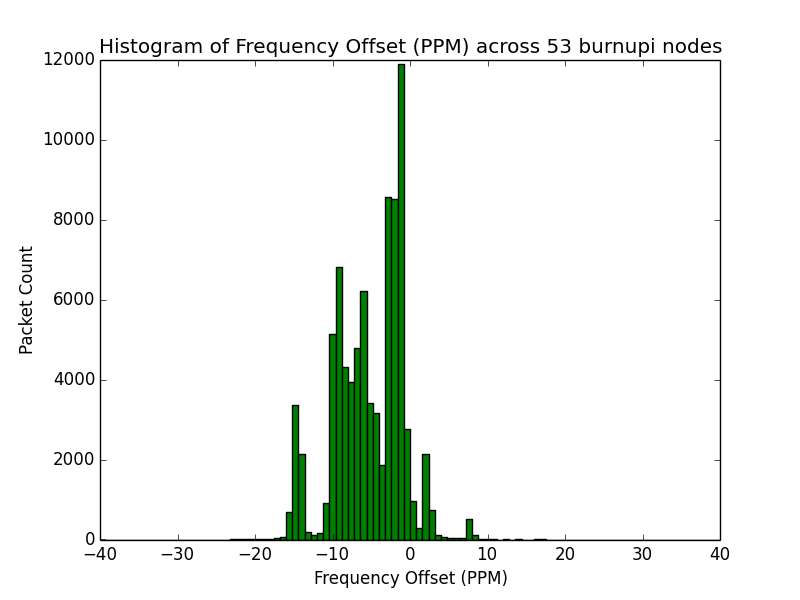
\includegraphics[width=0.8\textwidth]{burnupi-freq-offset.png}
\end{figure}

\begin{figure}[h]
  \centering
  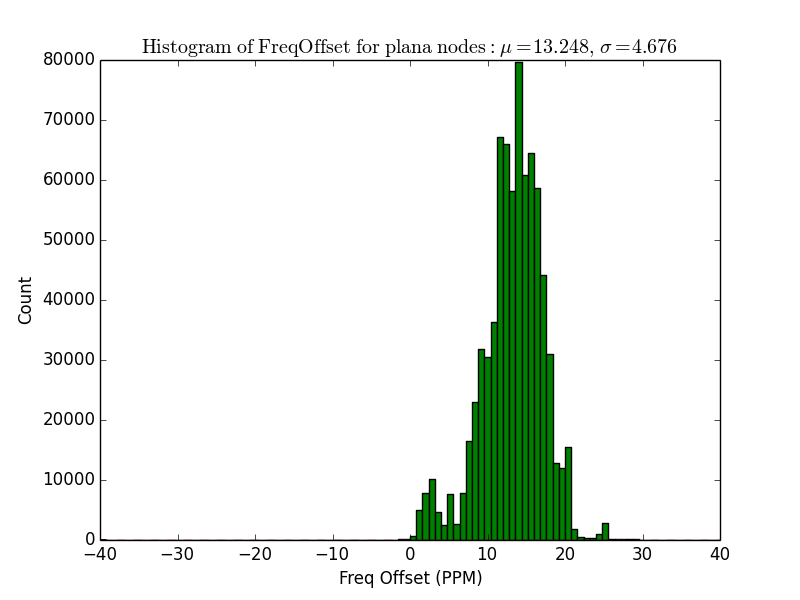
\includegraphics[width=0.8\textwidth]{plana-freq-offset.png}
\end{figure}

\section{Simulation of NTP for Performance and Analysis}

Although the recorded real-world statistics have been very useful for
understanding the behaviors of clocks and for validating our
understanding of time synchronization, real-world records are not
sufficient to be able to determine if our algorithm is correct. We
must also look at simulation results to be able to check that the
invariants that we would like to hold true do actually hold true. A
simulated network environment running on a single computer has the
advantage of having a single clock on which all simulated clocks are
based. By having a single clock, we are able to quantity and verify
the claims that time synchronization algorithms make about the quality
of a synchronization and the quality of the clocks involved.

By using a simulation that abstracts the clock from a physical clock,
we also eliminate any potential for idiosyncrasies of the host system
clock to affect the measurements gathered in the simulation. This has
the added benefit of allowing the simulation to run at a speed much
greater than real time.

We have chosen to use an environment called clknetsim <TODO citation> to
conduct our simulations. This choice was made for a variety of
reasons. Clknetsim is an open-source simulation package developed and
used by a major contributor to the chrony project <TODO citation> and the
linuxptp project <TODO citation> to test these protocol implementations. In
comparison to commercial network simulation products, It provides us
with a simple codebase and featureset targeted at our use case of
measuring time across a simulated network.

Clknetsim makes use of LDPRELOAD to intercept system calls that time
sychronization libraries make on their hosts. Using these intercepted
calls, clknetsim is able to monitor and capture the internal state of
the synchronization program. It is also able to fully control the
information the time library receives from the network and the system
clock. As clknetsim is in simulating system clocks and the network
connections, it can shape behavior of these components to test
different setups and hardware properties.
        
We are most interested in collecting and measuring two parameters in
this system. We first want to determine if the maximum uncertainty
reported by NTP is accurate. Clknetsim allows us to do this by, for a
given timestamp in the simulation, allowing us to observe what NTP
thinks the time is along with information about how certain NTP is
about that time. Our second goal is to analyze how low of an
uncertainty can be reached. As our algorithm is predicated on a upper
bound of the uncertainty in time, performance analysis can be
accomplished by observing how modifying various parameters affect the
maximum error term that NTP reports.

Over the course of our project, we have made slight additions to and
modifications of the clknetsim package. These modifications and
extensions are mostly superficial and made in order to expose state
parameters of NTP that were not previously being exposed, including
the maximum error term.
